\scanpage{13}
\mspage{6}
% archive foliation: 12
\uline{NB} L'ensemble produit à 4 éléments
\[
\deleted{\unsure{\underline{\omega}_Q}} C\times D
\]
peut s'identifier à l'ensemble quotient $R/\underline{a}$ des repères du carré
$Q$, modulo antipodisme
\[
 C\times D\simeq R/\underline{a}
 \qquad R=\operatorname{Rep}_{\unsure{\circ|0}}(Q)\simeq\operatorname{Rep}(Q^\circ)
\]
\margin{\figure{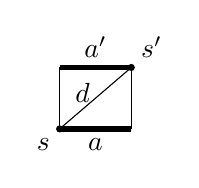
\begin{tikzpicture}[scale=.65]
\draw (0,0) rectangle (1.4,1.2);
\draw[line width=2pt] (0,0)--(1.4,0) (0,1.2)--(1.4,1.2);
\draw (0,0)--(1.4,1.2);
\fill (0,0) circle (2pt) (1.4,1.2) circle (2pt);
\node[below left] at (0,0) {$s$};
\node[above right] at (1.4,1.2) {$s'$};
\node[above] at (.7,1.2) {$a'$};
\node[below] at (.7,0) {$a$};
\node at (.45,.7) {$d$};
\end{tikzpicture}}}
tandis que $\underline{\omega}_Q$ s'identifie à
\deleted{l'ensemble} un ensemble de deux parties de $R$ (``$R^+$'' et ``$R^-$'')
complémentaires l'une de l'autre, et stables chacune par l'antipodisme
$\underline{a}$ (qui conserve l'orientation), ce qui fait que le choix d'un
élément de $R/\underline{a}$ définit canoniquement une orientation de $Q$,
\deleted{\unsure{un}} i.e. un des deux \deleted{\unsure{sous-ens.}} ens. de
repères $R',R''$.
Pour vérifier que à cette description d'une isom.
$C\wedge D\simeq\underline{\omega}_Q$ i.e. d'une relation
$\underline{\omega}_Q\wedge C\wedge D\simeq1$ correspond à
\deleted{\unsure{$\varpi\wedge c\wedge d=0$}}\inserted{$\varpi c d=1$},
il faut expliciter d'abord les conventions qui nous
\deleted{font} conduisent aux plongements
\[
 C\hookrightarrow V_S\setminus\{1,\underline{a}\}\subset\mathfrak{D},
 \qquad D\hookrightarrow V_A\setminus\{1,\underline{a}\}\subset\mathfrak{D},
 \qquad \underline{\omega}_Q\subset\mathfrak{D}^+\subset\mathfrak{D}
\]
Si $c$ est une \inserted{codiagonale i.e.} paire de côtés opposés du carré,
je vais lui associer l'autom. $g$ du carré qui fixe ces deux côtés
et qui échange les deux autres i.e. la symétrie p.r. à l'axe transversal.
De même, pour une diagonale, je lui associe la symétrie par rapport à cette
diagonale. Pour une orientation définie par un repère
\deleted{\unsure{ce}}
\figure{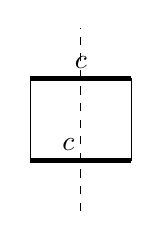
\begin{tikzpicture}[scale=.8]
\draw (0,0) rectangle (1.6,1.3);
\draw[line width=2pt] (0,0)--(1.6,0) (0,1.3)--(1.6,1.3);
\draw[dashed] (.8,-.8)--(.8,2.1);
\node[above] at (.8,1.3) {$c$};
\node[above] at (.6,0) {$c$};
\end{tikzpicture}
\qquad
\begin{tikzpicture}[scale=.8]
\draw[dashed] (0,0) rectangle (1.6,1.3);
\draw[dashed] (-.65,-.53)--(2.1,1.71);
\node[left] at (0,0) {$d$};
\node[above left] at (1.6,1.3) {$d$};
\end{tikzpicture}}
